\section{Measurement study}\label{sec:prediction}
In this section we conduct an extensive measurement study using network traces from a large cellular service provider to show the predictability of a few key performance metrics that affects available throughput. The traces are collected for 5 minutes in June 2014 from several locations in the United States. The data covers more than half million users distributed over 2000 eNodeBs. The following KPIs were monitored
\begin{table}[htbf]
\centering
\begin{tabular}{l|c|c|}
Metric & Description & Resolution \\ \hline
CQI & Channel Quality Indicator & 1 sec \\
RSRQ & Pilot Signal quality & 1sec \\
RRC & Radio resource connections & 1 min \\
HO & Hand over & 1 min \\
Tput & Throughput & ? \\ \hline
\end{tabular}
\caption{Key Performance Indicators in LTE network}
\end{table}


%Proportional fair schedulers have been widely deployed in 3G and 4G networks to achieve high spectrum efficiency. It takes the channel conditions and the number of active users as inputs and schedules packets accordingly. In this section, we study how accurate prediction can give us for the two key inputs-channel condition and the number of active users. The information can be mapped to an available throughput, however we have not fully explored the underline relation between them. This approach is different from end-to-end monitoring approaches as it does not require constantly saturating the link to get the maximum bandwidth. 


\begin{comment}
\subsection{Proportional Fair Scheduler}\label{subsec:ltenet}
3G ad 4G networks are using Orthogonal Frequency-Division Multiuser Access(OFDMA) scheme to achieve high spectrum efficiency. To achieve multiuser diversity, NodeBs and eNodeBs are running variations of proportional fair scheduling system. A basic \textit{proportional fair scheduler} works as the following: eNodeBs obtain the feedback from each user about their instantaneous channel quality conditions (CQ) in terms of encoding rate per resource block, and take the ratio between it and historical mean of CQ and pick the user with the maximum ratio. In a static model over a long term, each user will get 1/N share of resource blocks if N is the static number of users in the cell, a dynamic model also has a similar result\cite{PFINFOCOM}. The maximum bandwidth for each user in a cell is a function of: $T$-number of resource blocks in the cell, $N$-number of users in the cell, and $\mathbf{CQ}$-channel quality vector for all users; so maximum bandwidth vector for all users $\mathbf{BW} = f(T, N, \mathbf{CQ})$. We do not directly address $f(T, N, \mathbf{CQ})$ function in this paper as it is a vendor-specific PF-based scheduler. In the rest of the paper we assume a simple PF scheduler model, that is $\mathbf{BW} = f(T, N, \mathbf{CQ})=\frac{T}{N}*\mathbf{CQ}$. Among the three variables, $T$ is predetermined by the hardware, $N$ and $\mathbf{CQ}$ are the two factors we need to predict. 
\end{comment}


\subsection{Predictability}
We look at representative metrics and perform prediction over different lookahead horizons. The prediction accuracy is determined using standard statistical tools such as Mean Absolute Percentage Error (MAPE), Mean Square Percentage Error (MSPE). We also use the Cumulative Forecast Error (CFE), to indicate how the prediction deviates over a long duration. 

\begin{figure}[t]

\begin{minipage} {\linewidth}
\centering
 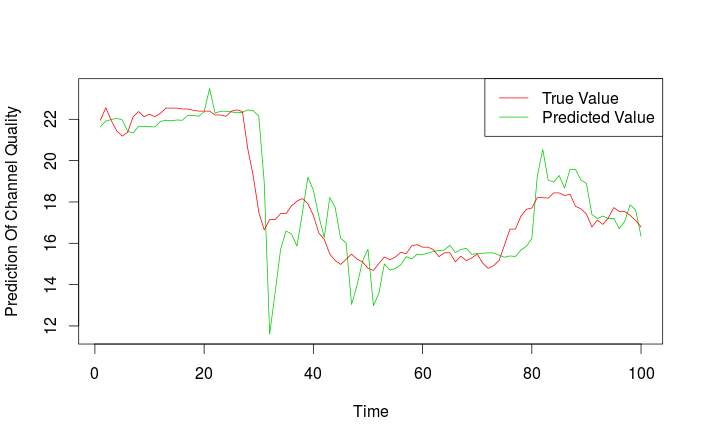
\includegraphics[width=\linewidth]{pictures/prediction.png}
\end{minipage}
\hspace{0.5cm}
\begin{minipage} {\linewidth}
\centering
 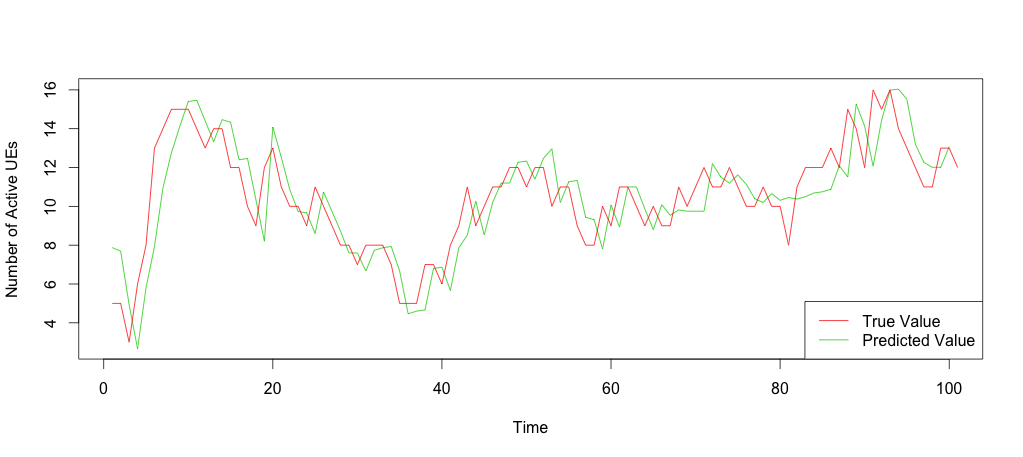
\includegraphics[width=\linewidth]{pictures/UE.png}
\end{minipage}

\caption{Predicting channel quality and active number of users} \label{fig:prediction}
\end{figure}

\subsection{Channel Quality}\label{subsec:CQ}
One unique characteristic for cellular network is the high mobility and this causes the link quality to fluctuate. Channel Quality Index is reported by the UE to inform the eNB about its signal quality~\cite{cqi}.  CQI ranges from 1 through 15. 

\emph{RSRQ:} Reference Signal Received Quality, is a key metric for the LTE wireless channel. RSRQ senses the load from other users in the same cell and the neighboring cells, and is indexed in 0-34 integer numbers; a higher number indicates a better link quality. RSRQ values can be mapped to certain encoding rate.

We predict the future RSRQ using time series analysis, in particular we use ARIMA (Auto-Regressive Integrated Moving Average) model to predict the next second: the algorithm fits the best ARIMA with historical data, and it uses a sliding window as the training dataset. We set window size to 15s. (We tried longer window but see no significant improvement over accuracy.) 

Through replaying 113 sample traces where the UEs are active for more than 100 seconds, we found that MAPE$<0.18$ for all the users, and the mean value is $0.064$. CFE values varies more across users with a maximum CFE=34.6, this is about three times of a unit value. In other words, for a 100 seconds prediction, prediction result may be 97\% accurate over long term and 82\% accurate on average for each prediction. 

The above results tell us that a simple prediction model such as ARIMA can offer a fairly accurate prediction. 

\subsection{Cell Load}\label{subsec:NUser}
We measured the number of active users in each cell from the same trace as mentioned above. The trace is collected from UE's RSRQ reports to eNodeBs. We assume a user is active in a certain second if the user reports RSRQ in a one-second interval. 

We apply ARIMA model, and find in most cases a random-walk model fits in the best. Different cells have different load, and the prediction works better in a heavily loaded cell. Since the inverse value of the active user number has a strong correlation with available bandwidth for each user, we take the inverse value to compute MAPE. For heavily loaded cell ($>30$ UEs) we have MAPE$<0.1$, and medium loaded cell (5-30 UEs) MAPE$<0.3$. This tells us we can achieve 70\% accuracy for each prediction on average for a medium to heavily loaded cell. For a lightly loaded cell, the prediction is not very satisfying, with MAPE$>1$. This is because the prediction value are affected to a greater extent by the small true value. However for a lightly loaded cell each user usually has higher available bandwidth, and thus has less need for extra information such as the available bandwidth.  

\begin{comment}

\section{Design} \label{sec:optimization}
In this section, we explain the reason to choose an \textbf{\emph{end-to-end decision making with in-network knowledge}} model in section \ref{designchoice}, we then explain the our architecture in section \ref{architecture}. 
%introduce performance metrics in section \ref{metrics} and 

\subsection{Who decides the video streaming?}\label{designchoice}
For video streaming service decision making, there are three different models: \emph{In-network}, \emph{strictly end-to-end} and \emph{End-to-end with in-network knowledge}. 

\emph{In-network techniques} make decisions for users: it selects the video bit rate and schedule the download for users based on its knowledge of the network condition. However in-network approaches lack the insight of the video play progress, e.g., video buffer occupancy since it does not deal with any video decoding. Aside from technical reasons, here are several privacy/policy reasons for not doing this: most content providers are using encrypted http connections which ISPs cannot access; users may be concerned about their data budgets and thus not choose high bit rate; or content providers have different video play bit rate policies for different users based on their subscription contracts. 

\emph{End-to-end techniques} probe the network condition based on round trip time (RTT) and historical throughput, however existence of the proxy makes the RTT very inaccurate as it splits tcp connections. The dynamic nature of the wireless link makes historical data unable to capture the link behavior, e.g. the available bandwidth may plummet due to fading effects or handoff and recovers very soon after, current end-to-end approaches fail to react to those scenarios in most cases.

\emph{End-to-end with in-network knowledge} model addresses the above issues: instead of making the decision for the client; the network helps video streaming service make better decisions via offering some key performance metrics about the network condition, such as available throughput and handoff. 

Though an end-to-end with in-network knowledge approach has advantages over the other two, we still need to address the problem of how to expose the in-network knowledge in a least intrusive way in a scalable manner. 







\subsection{Architecture}\label{architecture}

We propose a two-tiered system for to implement OpenCell system. The two parts sit in RAN and EPC respectively. 

At the lower tier we have bandwidth estimator for each eNodeB. Estimating link channel quality and cell load is much more scalable if if we compute it at eNodeBs, since there are only hundreds of users at each cell, while aggregated number of users for a SGW can be tens of thousands. Making an estimation at second level means for each user the computational cycle is ~1 $ms$ if sitting at eNodeBs and ~10  $\mu s$ if sitting at Serving Gateway. Processing the raw information such as RSRQ from eNodeBs and extract it as estimated bandwidth also reduces the extra traffic generated for message passing. 

At the higher tier, the information inferred at eNodeBs are received at the proxy, and combined with handoff information, we make a final estimation of available bandwidth for each user and then expose this piece of information to application service providers by some means. The architecture is in figure \ref{cellular}.

\begin{figure}[t]\label{cellular}
\begin{minipage}[b]{\linewidth}
\centering
 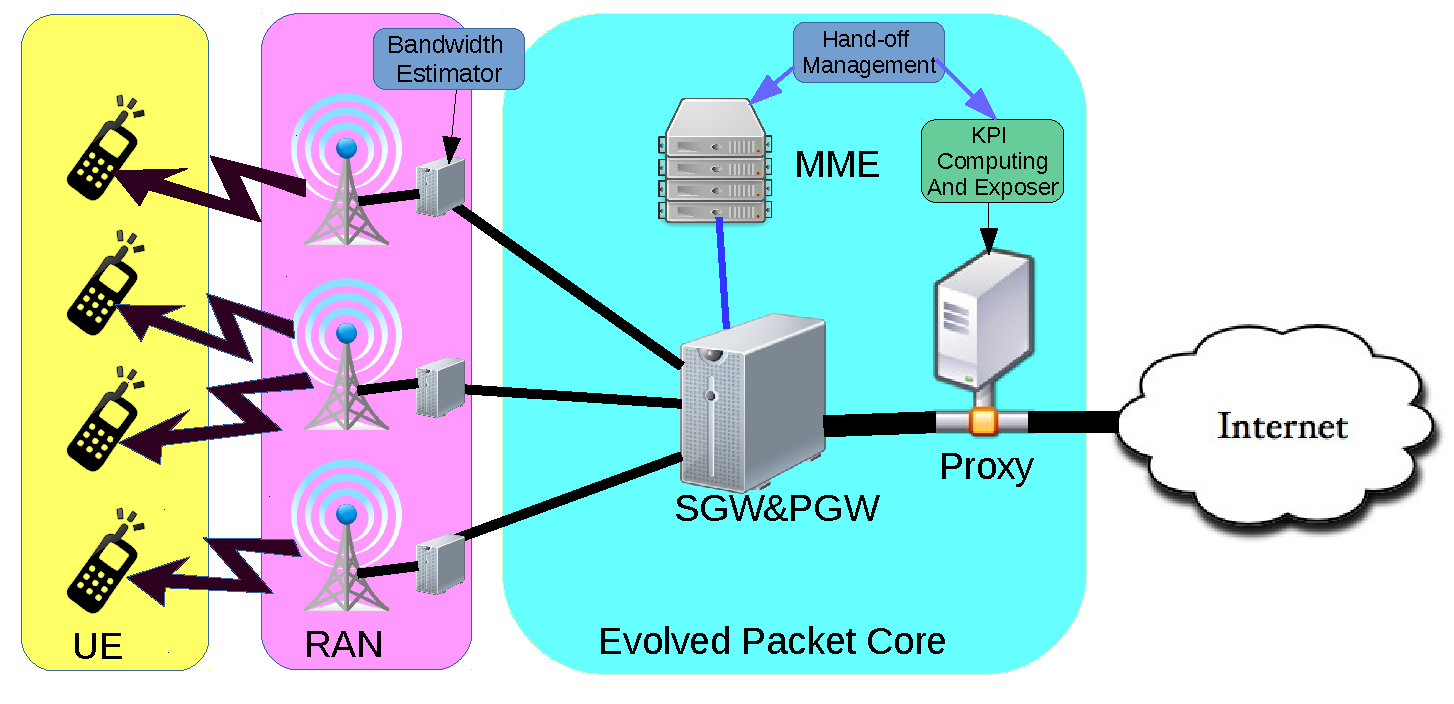
\includegraphics[width=\linewidth]{cellular.pdf}
\end{minipage}
\caption{OpenCell Design}
\end{figure}

In terms of how to expose the API information, there are three options: encapsulation (i) at TCP/IP layer, (ii) at application layer; and (iii) using a distinct channel. Each approach has its pros and cons, for example TCP/IP layer does not require DPI but the fields used for encapsulation might be overwritten deep in the network from middleboxes. Using distinct channel does not suffer either problem but it requires application service providers' cooperation. We are still weighing between the options and leave this as a future problem. 



\end{comment}
